\begin{figure}[h!]
\centering

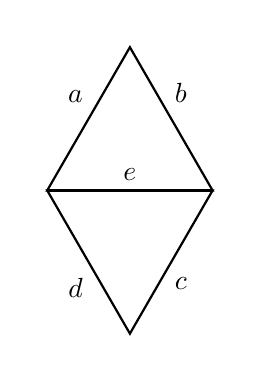
\begin{tikzpicture}[scale=0.7, baseline, thick]

    \draw (0,0)--(3,0)--(60:3)--cycle;
    \draw (0,0)--(3,0)--(-60:3)--cycle;

    \draw (0,0) -- (3,0);

    \draw node[above]      at (70:1.5){$a$};
    \draw node[above]      at (30:2.8){$b$};
    \draw node[below]      at (-30:2.8){$c$};
    \draw node[below=-0.1] at (-70:1.5){$d$};
    \draw node[above] at (1.5, 0){$e$};

    \draw node[left] at (0,0) {};
    \draw node[above] at (60:3) {};
    \draw node[right] at (3,0) {};
    \draw node[below] at (-60:3) {};

\end{tikzpicture}
\begin{tikzpicture}[baseline]
    \draw[->, thick](0,0)--(1,0);
    \node[above]  at (0.5,0) {};
\end{tikzpicture}
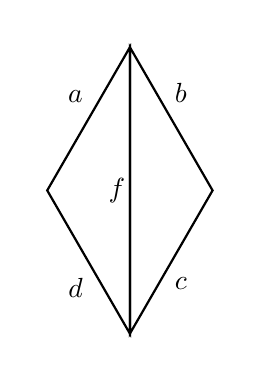
\begin{tikzpicture}[scale=0.7, baseline, thick,every node/.style={sloped,allow upside down}]
    \draw (0,0)--(60:3)--(-60:3)--cycle;
    \draw (3,0)--(60:3)--(-60:3)--cycle;

    \draw node[above]      at (70:1.5)  {$a$};
    \draw node[above]      at (30:2.8)  {$b$};
    \draw node[below]      at (-30:2.8) {$c$};
    \draw node[below=-0.1] at (-70:1.5) {$d$};
    \draw node[left]       at (1.6,0)   {$f$};

    \draw (1.5,-2) --  (1.5,2);

    \draw node[left] at (0,0) {};
    \draw node[above] at (60:3) {};
    \draw node[right] at (3,0) {};
    \draw node[below] at (-60:3) {};

\end{tikzpicture}
\caption{Ptolemy transformation.}\label{fig:ptolemy}
\end{figure}
